\section{General Structure}

The Lambda architecture precomputes specific data structures for answering particular queries.
This is because of the large amount of data and complexity of algorithms.
These data structures are called \textit{views}\mnote{view}.
They store aggregations of the original data and result of execution of classification or other algorithms.

There are two approaches of preparing views.
The first one is to do it in a batch mode considering all available data for computations.
The second one is to construct views incrementally in the real time with newly arrived data.
Together these two methods give an opportunity to answer queries fast and accurate.
Figure~\ref{fig:lambda_architecture} depicts how the Lambda architecture combines batch and incremental processing to answer queries.
Batch and serving layer are responsible for batch views, speed layer provides real-time views.
To answer query system merges data from both types of views.

\begin{figure}[h]
  \centering
  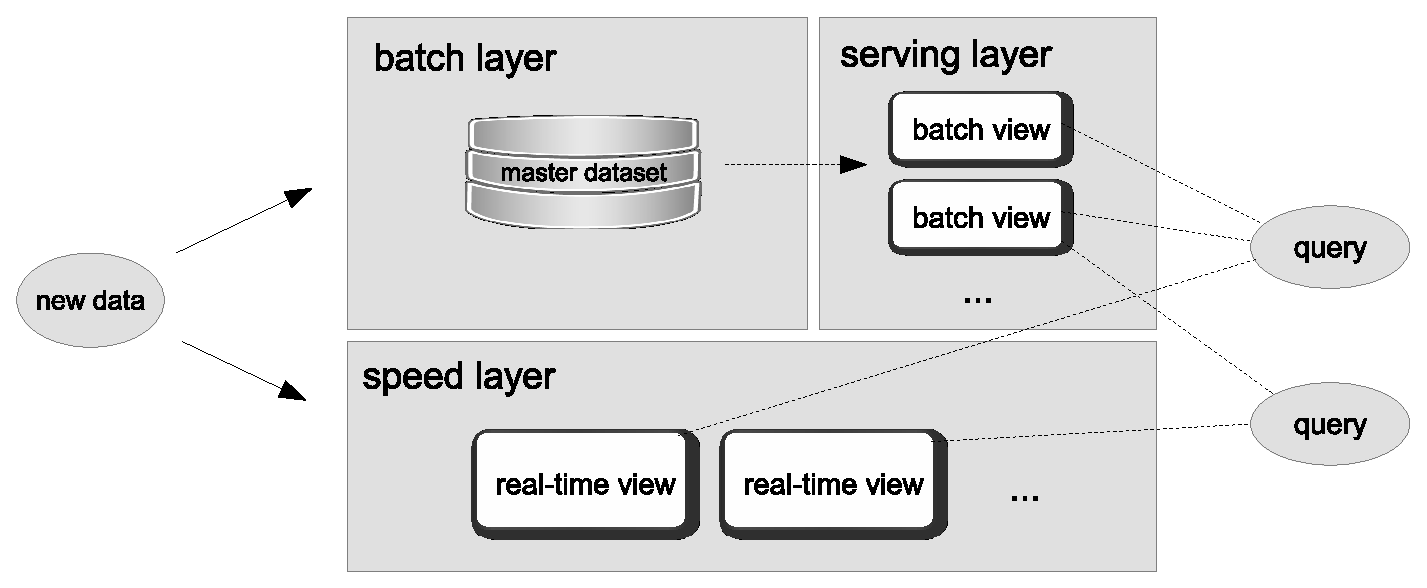
\includegraphics [width=1.0\textwidth]{images/LambdaArchitecture}
  \caption{General structure of the Lambda architecture.}
  \label{fig:lambda_architecture}
\end{figure}

The \textit{batch layer} \mnote{batch layer} of the Lambda architecture is responsible for batch processing.
It takes the whole dataset and executes batch computations on it.
Views, that are the result of the batch processing, are called \textit{batch views}\mnote{batch view}.
This operation is efficient, because all data is at once in disposal.
We can execute any algorithm, and produce any kind of index or aggregation.
It is also easy to program using such great batch processing approaches as MapReduce.
This paradigm is inherently distributed and scalable, what allows to use hundreds and thousands of machines for batch processing.

After the batch layer has precomputed views, it places them into the \textit{serving layer}\mnote{serving layer}.
The serving layer is responsible for storage of batch views.
It also creates indices on those views and provides interfaces to get particular data records from them.

Batch layer starts then computations again, considering now data, that has come during the last batch processing.
This loop goes on infinitely.
Batch processing always starts again from scratch using all data, available to the moment of its start.
When the batch layer stores computed views into the serving layer, it discards old ones.

Batch computations, although easy and efficient, take long time to be done.
This cannot be underestimated, because on the BigData scale computations can last hours even if we setup cluster of thousands of machines.

As long as batch computations take much time, views are always outdated for several hours.
During this time new data arrives to the system, and it must be also counted in query answers.
This is not possible to solve using only batch processing.
Therefore, another approach has to be applied.

To overcome delay of batch computations the Lambda architecture has additional component - the \textit{speed layer}\mnote{speed layer}.
It also computes views, but in incremental fashion.
Such views are called \textit{real-time views}\mnote{real-time view}.
As new data arrives, the speed layer updates incrementally real-time views.
Hence, they always has information from data, gathered during current batch processing.
When batch processing finishes and old batch views are replaced by new, the speed layer drops real-time views and starts to accumulate them from the beginning.

Finally, to answer queries system uses both batch and real-time views.
Batch views contain result of the last batch processing.
Real-time views provide information from data, gathered after the beginning of the current batch processing.
Merging both types of views, system produces accurate and actual answers to the queries.